\documentclass[twoside]{book}

% Packages required by doxygen
\usepackage{fixltx2e}
\usepackage{calc}
\usepackage{doxygen}
\usepackage[export]{adjustbox} % also loads graphicx
\usepackage{graphicx}
\usepackage[utf8]{inputenc}
\usepackage{makeidx}
\usepackage{multicol}
\usepackage{multirow}
\PassOptionsToPackage{warn}{textcomp}
\usepackage{textcomp}
\usepackage[nointegrals]{wasysym}
\usepackage[table]{xcolor}

% Font selection
\usepackage[T1]{fontenc}
\usepackage[scaled=.90]{helvet}
\usepackage{courier}
\usepackage{amssymb}
\usepackage{sectsty}
\renewcommand{\familydefault}{\sfdefault}
\allsectionsfont{%
  \fontseries{bc}\selectfont%
  \color{darkgray}%
}
\renewcommand{\DoxyLabelFont}{%
  \fontseries{bc}\selectfont%
  \color{darkgray}%
}
\newcommand{\+}{\discretionary{\mbox{\scriptsize$\hookleftarrow$}}{}{}}

% Page & text layout
\usepackage{geometry}
\geometry{%
  a4paper,%
  top=2.5cm,%
  bottom=2.5cm,%
  left=2.5cm,%
  right=2.5cm%
}
\tolerance=750
\hfuzz=15pt
\hbadness=750
\setlength{\emergencystretch}{15pt}
\setlength{\parindent}{0cm}
\setlength{\parskip}{3ex plus 2ex minus 2ex}
\makeatletter
\renewcommand{\paragraph}{%
  \@startsection{paragraph}{4}{0ex}{-1.0ex}{1.0ex}{%
    \normalfont\normalsize\bfseries\SS@parafont%
  }%
}
\renewcommand{\subparagraph}{%
  \@startsection{subparagraph}{5}{0ex}{-1.0ex}{1.0ex}{%
    \normalfont\normalsize\bfseries\SS@subparafont%
  }%
}
\makeatother

% Headers & footers
\usepackage{fancyhdr}
\pagestyle{fancyplain}
\fancyhead[LE]{\fancyplain{}{\bfseries\thepage}}
\fancyhead[CE]{\fancyplain{}{}}
\fancyhead[RE]{\fancyplain{}{\bfseries\leftmark}}
\fancyhead[LO]{\fancyplain{}{\bfseries\rightmark}}
\fancyhead[CO]{\fancyplain{}{}}
\fancyhead[RO]{\fancyplain{}{\bfseries\thepage}}
\fancyfoot[LE]{\fancyplain{}{}}
\fancyfoot[CE]{\fancyplain{}{}}
\fancyfoot[RE]{\fancyplain{}{\bfseries\scriptsize Generated by Doxygen }}
\fancyfoot[LO]{\fancyplain{}{\bfseries\scriptsize Generated by Doxygen }}
\fancyfoot[CO]{\fancyplain{}{}}
\fancyfoot[RO]{\fancyplain{}{}}
\renewcommand{\footrulewidth}{0.4pt}
\renewcommand{\chaptermark}[1]{%
  \markboth{#1}{}%
}
\renewcommand{\sectionmark}[1]{%
  \markright{\thesection\ #1}%
}

% Indices & bibliography
\usepackage{natbib}
\usepackage[titles]{tocloft}
\setcounter{tocdepth}{3}
\setcounter{secnumdepth}{5}
\makeindex

% Hyperlinks (required, but should be loaded last)
\usepackage{ifpdf}
\ifpdf
  \usepackage[pdftex,pagebackref=true]{hyperref}
\else
  \usepackage[ps2pdf,pagebackref=true]{hyperref}
\fi
\hypersetup{%
  colorlinks=true,%
  linkcolor=blue,%
  citecolor=blue,%
  unicode%
}

% Custom commands
\newcommand{\clearemptydoublepage}{%
  \newpage{\pagestyle{empty}\cleardoublepage}%
}

\usepackage{caption}
\captionsetup{labelsep=space,justification=centering,font={bf},singlelinecheck=off,skip=4pt,position=top}

%===== C O N T E N T S =====

\begin{document}

% Titlepage & ToC
\hypersetup{pageanchor=false,
             bookmarksnumbered=true,
             pdfencoding=unicode
            }
\pagenumbering{alph}
\begin{titlepage}
\vspace*{7cm}
\begin{center}%
{\Large Theia }\\
\vspace*{1cm}
{\large Generated by Doxygen 1.8.13}\\
\end{center}
\end{titlepage}
\clearemptydoublepage
\pagenumbering{roman}
\tableofcontents
\clearemptydoublepage
\pagenumbering{arabic}
\hypersetup{pageanchor=true}

%--- Begin generated contents ---
\chapter{Hierarchical Index}
\section{Class Hierarchy}
This inheritance list is sorted roughly, but not completely, alphabetically\+:\begin{DoxyCompactList}
\item \contentsline{section}{Command\+Args}{\pageref{classCommandArgs}}{}
\item \contentsline{section}{Descent\+Functor}{\pageref{classDescentFunctor}}{}
\item \contentsline{section}{Efficiency\+Vector}{\pageref{classEfficiencyVector}}{}
\item \contentsline{section}{File}{\pageref{structFile}}{}
\item \contentsline{section}{File\+Star\+Pairs}{\pageref{structFileStarPairs}}{}
\item \contentsline{section}{Likelihood\+Data}{\pageref{classLikelihoodData}}{}
\item \contentsline{section}{Log\+Likelihood}{\pageref{classLogLikelihood}}{}
\begin{DoxyCompactList}
\item \contentsline{section}{Log\+Likelihood\+Prior}{\pageref{classLogLikelihoodPrior}}{}
\end{DoxyCompactList}
\item \contentsline{section}{Memory\+Buffer}{\pageref{structMemoryBuffer}}{}
\item \contentsline{section}{Optimiser\+Properties}{\pageref{structOptimiserProperties}}{}
\item \contentsline{section}{Optimiser\+Status}{\pageref{structOptimiserStatus}}{}
\item \contentsline{section}{Optimizer$<$ T $>$}{\pageref{classOptimizer}}{}
\item \contentsline{section}{Progress\+Tracker}{\pageref{structProgressTracker}}{}
\item \contentsline{section}{Star}{\pageref{classStar}}{}
\item \contentsline{section}{Stop\+Conditions}{\pageref{structStopConditions}}{}
\item \contentsline{section}{Variance\+Population}{\pageref{structVariancePopulation}}{}
\end{DoxyCompactList}

\chapter{Class Index}
\section{Class List}
Here are the classes, structs, unions and interfaces with brief descriptions\+:\begin{DoxyCompactList}
\item\contentsline{section}{\hyperlink{classCommandArgs}{Command\+Args} }{\pageref{classCommandArgs}}{}
\item\contentsline{section}{\hyperlink{classDescentFunctor}{Descent\+Functor} }{\pageref{classDescentFunctor}}{}
\item\contentsline{section}{\hyperlink{classEfficiencyVector}{Efficiency\+Vector} }{\pageref{classEfficiencyVector}}{}
\item\contentsline{section}{\hyperlink{structFile}{File} }{\pageref{structFile}}{}
\item\contentsline{section}{\hyperlink{structFileStarPairs}{File\+Star\+Pairs} }{\pageref{structFileStarPairs}}{}
\item\contentsline{section}{\hyperlink{classLikelihoodData}{Likelihood\+Data} }{\pageref{classLikelihoodData}}{}
\item\contentsline{section}{\hyperlink{classLogLikelihood}{Log\+Likelihood} }{\pageref{classLogLikelihood}}{}
\item\contentsline{section}{\hyperlink{classLogLikelihoodPrior}{Log\+Likelihood\+Prior} }{\pageref{classLogLikelihoodPrior}}{}
\item\contentsline{section}{\hyperlink{structMemoryBuffer}{Memory\+Buffer} }{\pageref{structMemoryBuffer}}{}
\item\contentsline{section}{\hyperlink{structOptimiserProperties}{Optimiser\+Properties} }{\pageref{structOptimiserProperties}}{}
\item\contentsline{section}{\hyperlink{structOptimiserStatus}{Optimiser\+Status} }{\pageref{structOptimiserStatus}}{}
\item\contentsline{section}{\hyperlink{classOptimizer}{Optimizer$<$ T $>$} }{\pageref{classOptimizer}}{}
\item\contentsline{section}{\hyperlink{structProgressTracker}{Progress\+Tracker} }{\pageref{structProgressTracker}}{}
\item\contentsline{section}{\hyperlink{classStar}{Star} }{\pageref{classStar}}{}
\item\contentsline{section}{\hyperlink{structStopConditions}{Stop\+Conditions} }{\pageref{structStopConditions}}{}
\item\contentsline{section}{\hyperlink{structVariancePopulation}{Variance\+Population} }{\pageref{structVariancePopulation}}{}
\end{DoxyCompactList}

\chapter{Class Documentation}
\hypertarget{classCommandArgs}{}\section{Command\+Args Class Reference}
\label{classCommandArgs}\index{Command\+Args@{Command\+Args}}
\subsection*{Public Member Functions}
\begin{DoxyCompactItemize}
\item 
\mbox{\Hypertarget{classCommandArgs_a93f101d465df0ff6e79950c6b8ac4cd5}\label{classCommandArgs_a93f101d465df0ff6e79950c6b8ac4cd5}} 
void {\bfseries Read\+Arguments} (int argc, char $\ast$argv\mbox{[}$\,$\mbox{]}, int Process\+Rank)
\end{DoxyCompactItemize}
\subsection*{Data Fields}
\begin{DoxyCompactItemize}
\item 
\mbox{\Hypertarget{classCommandArgs_a7227f10097dae1825feea951fc3132a6}\label{classCommandArgs_a7227f10097dae1825feea951fc3132a6}} 
Argument$<$ int $>$ {\bfseries Random\+Seed} = Argument$<$int$>$(0,\char`\"{}random-\/seed\char`\"{})
\item 
\mbox{\Hypertarget{classCommandArgs_acaf9e3be3c41eeb7f3fe61d26312a0ad}\label{classCommandArgs_acaf9e3be3c41eeb7f3fe61d26312a0ad}} 
Argument$<$ std\+::string $>$ {\bfseries Start\+Vector\+Location} = Argument$<$std\+::string$>$(\char`\"{}\+\_\+\+\_\+null\+\_\+location\+\_\+\+\_\+\char`\"{},\char`\"{}restart\char`\"{})
\item 
\mbox{\Hypertarget{classCommandArgs_a47a53ea373bc6c81ed80c2b651e9c405}\label{classCommandArgs_a47a53ea373bc6c81ed80c2b651e9c405}} 
Argument$<$ double $>$ {\bfseries Grad\+Lim} = Argument$<$double$>$(0,\char`\"{}gradlim\char`\"{})
\item 
\mbox{\Hypertarget{classCommandArgs_a9d8b6a8c21f7b330979c7a173994ca37}\label{classCommandArgs_a9d8b6a8c21f7b330979c7a173994ca37}} 
Argument$<$ int $>$ {\bfseries Max\+Steps} = Argument$<$int$>$(1000,\char`\"{}max-\/steps\char`\"{})
\item 
\mbox{\Hypertarget{classCommandArgs_aedd3311893f45b92b4a7f598792f7f2e}\label{classCommandArgs_aedd3311893f45b92b4a7f598792f7f2e}} 
Argument$<$ int $>$ {\bfseries Freeze\+Steps} = Argument$<$int$>$(0,\char`\"{}burnin\char`\"{})
\item 
\mbox{\Hypertarget{classCommandArgs_af906f01863ff7b503914b462a8a7ddb5}\label{classCommandArgs_af906f01863ff7b503914b462a8a7ddb5}} 
Argument$<$ int $>$ {\bfseries Save\+Steps} = Argument$<$int$>$(1,\char`\"{}save-\/steps\char`\"{})
\item 
\mbox{\Hypertarget{classCommandArgs_ad1018830dc6772a972df87a843059416}\label{classCommandArgs_ad1018830dc6772a972df87a843059416}} 
Argument$<$ bool $>$ {\bfseries Save\+All\+Steps} = Argument$<$bool$>$(false,\char`\"{}unique-\/temp-\/save\char`\"{})
\item 
\mbox{\Hypertarget{classCommandArgs_ad16d6cadaedb80e8d3abfc51b3b73335}\label{classCommandArgs_ad16d6cadaedb80e8d3abfc51b3b73335}} 
Argument$<$ int $>$ {\bfseries Minibatches} = Argument$<$int$>$(64,\char`\"{}minibatch\char`\"{})
\item 
\mbox{\Hypertarget{classCommandArgs_ae64dd25052a877832d3db4e289f1bb13}\label{classCommandArgs_ae64dd25052a877832d3db4e289f1bb13}} 
Argument$<$ double $>$ {\bfseries Harness\+Slow\+Down} = Argument$<$double$>$(10,\char`\"{}harness-\/slow\char`\"{})
\item 
\mbox{\Hypertarget{classCommandArgs_a2a92d19a8106254917659b8d432b8fd2}\label{classCommandArgs_a2a92d19a8106254917659b8d432b8fd2}} 
Argument$<$ int $>$ {\bfseries Harness\+Release} = Argument$<$int$>$(5,\char`\"{}harness-\/release\char`\"{})
\item 
\mbox{\Hypertarget{classCommandArgs_a5e4469cda4fd80e0d827a11147b15afa}\label{classCommandArgs_a5e4469cda4fd80e0d827a11147b15afa}} 
Argument$<$ std\+::string $>$ {\bfseries Data\+Source} = Argument$<$std\+::string$>$(\char`\"{}../../Data/Shuffled\+Data\char`\"{},\char`\"{}data\char`\"{})
\item 
\mbox{\Hypertarget{classCommandArgs_adf5dd695a6a88eed97d1317d534af4d6}\label{classCommandArgs_adf5dd695a6a88eed97d1317d534af4d6}} 
Argument$<$ std\+::string $>$ {\bfseries Output\+Directory} = Argument$<$std\+::string$>$(\char`\"{}Output\char`\"{},\char`\"{}output\char`\"{})
\item 
\mbox{\Hypertarget{classCommandArgs_ab0522bf4c5550780b9ff929fbc272f72}\label{classCommandArgs_ab0522bf4c5550780b9ff929fbc272f72}} 
std\+::vector$<$ J\+S\+L\+::\+Argument\+Interface $\ast$ $>$ {\bfseries arg\+Pointers} = \{\&Random\+Seed, \&Start\+Vector\+Location, \&Grad\+Lim, \&Max\+Steps, \&Freeze\+Steps, \&Data\+Source, \&Output\+Directory,\&Save\+Steps,\&Save\+All\+Steps,\&Minibatches,\&Harness\+Release,\&Harness\+Slow\+Down\}
\end{DoxyCompactItemize}


The documentation for this class was generated from the following file\+:\begin{DoxyCompactItemize}
\item 
/home/fraserj/\+Documents/\+Work/\+Gaia\+Selection\+Function/\+Code/\+Theia/src/\+Data\+Handling/Command\+Arguments.\+h\end{DoxyCompactItemize}

\hypertarget{classDescentFunctor}{}\doxysection{Descent\+Functor Class Reference}
\label{classDescentFunctor}\index{DescentFunctor@{DescentFunctor}}
\doxysubsection*{Public Member Functions}
\begin{DoxyCompactItemize}
\item 
\mbox{\Hypertarget{classDescentFunctor_a8d72ed3391cb867e5568ca2cc1b4c325}\label{classDescentFunctor_a8d72ed3391cb867e5568ca2cc1b4c325}} 
{\bfseries Descent\+Functor} (int n, const std\+::vector$<$ std\+::vector$<$ \mbox{\hyperlink{classStar}{Star}} $>$$>$ \&data, int n\+Params, std\+::string outdir, int n\+Stars, int max\+Batches, bool time\+Active, bool space\+Active, bool hyper\+Active)
\item 
\mbox{\Hypertarget{classDescentFunctor_a38f1c319b730f318c9ce89718e377ebf}\label{classDescentFunctor_a38f1c319b730f318c9ce89718e377ebf}} 
void {\bfseries Distribute\+Calculations} (const Vector\+Xd \&y, int batch\+ID, int effective\+Batches)
\item 
\mbox{\Hypertarget{classDescentFunctor_a0c3a1b76e6fce3713c6d6a8761ff1bf3}\label{classDescentFunctor_a0c3a1b76e6fce3713c6d6a8761ff1bf3}} 
void {\bfseries Calculate} (const Vector\+Xd \&x, int batch\+ID, int effective\+Batches)
\item 
\mbox{\Hypertarget{classDescentFunctor_acfae2cdc2983a8eb215fb334bcdb0863}\label{classDescentFunctor_acfae2cdc2983a8eb215fb334bcdb0863}} 
void {\bfseries Calculate} (const Vector\+Xd \&x)
\item 
\mbox{\Hypertarget{classDescentFunctor_a3de250a0703477a82312614785bcdb8b}\label{classDescentFunctor_a3de250a0703477a82312614785bcdb8b}} 
void {\bfseries Save\+Position} (bool final\+Save, int save\+Step, bool unique\+Save, const Vector\+Xd \&x)
\item 
\mbox{\Hypertarget{classDescentFunctor_a516e1d332b2ce3d3307e2ee67ee0b94f}\label{classDescentFunctor_a516e1d332b2ce3d3307e2ee67ee0b94f}} 
void {\bfseries Unfreeze} ()
\end{DoxyCompactItemize}
\doxysubsection*{Data Fields}
\begin{DoxyCompactItemize}
\item 
\mbox{\Hypertarget{classDescentFunctor_a14a7ae0eb78ad3a56a289ee300119104}\label{classDescentFunctor_a14a7ae0eb78ad3a56a289ee300119104}} 
int {\bfseries Loop\+ID}
\item 
\mbox{\Hypertarget{classDescentFunctor_a09bd6f8a2558a7530486ae0605f44983}\label{classDescentFunctor_a09bd6f8a2558a7530486ae0605f44983}} 
double {\bfseries Value}
\item 
\mbox{\Hypertarget{classDescentFunctor_acb32f6b34a3eb2d0ebf170a674ab1c02}\label{classDescentFunctor_acb32f6b34a3eb2d0ebf170a674ab1c02}} 
std\+::vector$<$ double $>$ {\bfseries Gradient}
\item 
\mbox{\Hypertarget{classDescentFunctor_a424da8de442d996ae9062bbedbcd7868}\label{classDescentFunctor_a424da8de442d996ae9062bbedbcd7868}} 
std\+::vector$<$ double $>$ {\bfseries mut\+\_\+gaps}
\item 
\mbox{\Hypertarget{classDescentFunctor_a80f4fb498c367c3bf9752163cb13f8f5}\label{classDescentFunctor_a80f4fb498c367c3bf9752163cb13f8f5}} 
std\+::vector$<$ double $>$ {\bfseries Frozen\+Space}
\item 
\mbox{\Hypertarget{classDescentFunctor_a2bddad96900bc85af34e773c092c257f}\label{classDescentFunctor_a2bddad96900bc85af34e773c092c257f}} 
std\+::vector$<$ double $>$ {\bfseries Frozen\+Time}
\item 
\mbox{\Hypertarget{classDescentFunctor_a8d0f68c56e365aa9d2a6804ea2627de8}\label{classDescentFunctor_a8d0f68c56e365aa9d2a6804ea2627de8}} 
std\+::vector$<$ double $>$ {\bfseries Frozen\+Hypers}
\end{DoxyCompactItemize}


The documentation for this class was generated from the following file\+:\begin{DoxyCompactItemize}
\item 
/home/jack/\+Documents/\+Work/\+Gaia\+Completeness/\+Code/\+Theia/src/\+Optimizer/Descent\+Functor.\+h\end{DoxyCompactItemize}

\hypertarget{classEfficiencyVector}{}\doxysection{Efficiency\+Vector Class Reference}
\label{classEfficiencyVector}\index{EfficiencyVector@{EfficiencyVector}}
\doxysubsection*{Data Fields}
\begin{DoxyCompactItemize}
\item 
\mbox{\Hypertarget{classEfficiencyVector_a138e823e4829aadd9e43b475848804cf}\label{classEfficiencyVector_a138e823e4829aadd9e43b475848804cf}} 
std\+::vector$<$ double $>$ {\bfseries Raw}
\item 
\mbox{\Hypertarget{classEfficiencyVector_af4687a6e7c72f35b35310e2368335b25}\label{classEfficiencyVector_af4687a6e7c72f35b35310e2368335b25}} 
std\+::vector$<$ double $>$ {\bfseries Transformed}
\end{DoxyCompactItemize}


The documentation for this class was generated from the following file\+:\begin{DoxyCompactItemize}
\item 
/home/jack/\+Documents/\+Work/\+Gaia\+Completeness/\+Code/\+Theia/src/\+Main/Efficiency\+Vector.\+h\end{DoxyCompactItemize}

\hypertarget{structFile}{}\section{File Struct Reference}
\label{structFile}\index{File@{File}}
\subsection*{Public Attributes}
\begin{DoxyCompactItemize}
\item 
\mbox{\Hypertarget{structFile_afcb65fdfafd4c6373b4c9d3e1ca9459d}\label{structFile_afcb65fdfafd4c6373b4c9d3e1ca9459d}} 
std\+::string {\bfseries Name}
\item 
\mbox{\Hypertarget{structFile_aced9c357d2c770816f23676e0a059d88}\label{structFile_aced9c357d2c770816f23676e0a059d88}} 
int {\bfseries Bin}
\end{DoxyCompactItemize}


The documentation for this struct was generated from the following file\+:\begin{DoxyCompactItemize}
\item 
/home/fraserj/\+Documents/\+Work/\+Gaia\+Selection\+Function/\+Code/\+Theia/src/\+Data\+Handling/Data\+Loading.\+h\end{DoxyCompactItemize}

\hypertarget{structFileStarPairs}{}\section{File\+Star\+Pairs Struct Reference}
\label{structFileStarPairs}\index{File\+Star\+Pairs@{File\+Star\+Pairs}}
\subsection*{Data Fields}
\begin{DoxyCompactItemize}
\item 
\mbox{\Hypertarget{structFileStarPairs_aec9230582e62f0acf8838794aea7e490}\label{structFileStarPairs_aec9230582e62f0acf8838794aea7e490}} 
std\+::string {\bfseries File\+Name}
\item 
\mbox{\Hypertarget{structFileStarPairs_a2c8e51cf299f1dbbf2e9d73614aee650}\label{structFileStarPairs_a2c8e51cf299f1dbbf2e9d73614aee650}} 
int {\bfseries N\+Stars}
\end{DoxyCompactItemize}


The documentation for this struct was generated from the following file\+:\begin{DoxyCompactItemize}
\item 
/home/fraserj/\+Documents/\+Work/\+Gaia\+Selection\+Function/\+Code/\+Theia/src/\+Data\+Handling/Data\+Loading.\+h\end{DoxyCompactItemize}

\hypertarget{classLikelihoodData}{}\section{Likelihood\+Data Class Reference}
\label{classLikelihoodData}\index{Likelihood\+Data@{Likelihood\+Data}}


{\ttfamily \#include $<$Data\+Storage.\+h$>$}

\subsection*{Public Member Functions}
\begin{DoxyCompactItemize}
\item 
\mbox{\Hypertarget{classLikelihoodData_abe754db1273e8ed99a0bf08a26c13aad}\label{classLikelihoodData_abe754db1273e8ed99a0bf08a26c13aad}} 
{\bfseries Likelihood\+Data} (const std\+::vector$<$ std\+::vector$<$ \hyperlink{classStar}{Star} $>$$>$ \&data, int id)
\item 
\mbox{\Hypertarget{classLikelihoodData_a1911a871964da019810ac0342352ae8c}\label{classLikelihoodData_a1911a871964da019810ac0342352ae8c}} 
void {\bfseries Generate\+Populations} (const std\+::vector$<$ double $>$ \&x)
\end{DoxyCompactItemize}
\subsection*{Data Fields}
\begin{DoxyCompactItemize}
\item 
\mbox{\Hypertarget{classLikelihoodData_a9cb6c7ac3a9bfb1c9108ead8ea8fde91}\label{classLikelihoodData_a9cb6c7ac3a9bfb1c9108ead8ea8fde91}} 
int {\bfseries ID}
\item 
\mbox{\Hypertarget{classLikelihoodData_a4c970663e2cd6c3e0b1a8e353854ce5f}\label{classLikelihoodData_a4c970663e2cd6c3e0b1a8e353854ce5f}} 
const std\+::vector$<$ std\+::vector$<$ \hyperlink{classStar}{Star} $>$ $>$ \& {\bfseries Stars}
\item 
\mbox{\Hypertarget{classLikelihoodData_a0c7b79c0856b8d63180245c7a423b262}\label{classLikelihoodData_a0c7b79c0856b8d63180245c7a423b262}} 
std\+::vector$<$ int $>$ {\bfseries healpix\+\_\+fov\+\_\+1}
\item 
\mbox{\Hypertarget{classLikelihoodData_a2caf37a2748bbb0bd91b818c3af51502}\label{classLikelihoodData_a2caf37a2748bbb0bd91b818c3af51502}} 
std\+::vector$<$ int $>$ {\bfseries healpix\+\_\+fov\+\_\+2}
\item 
\mbox{\Hypertarget{classLikelihoodData_ab996d0af29ea194954e9ddfeba2bea9e}\label{classLikelihoodData_ab996d0af29ea194954e9ddfeba2bea9e}} 
std\+::vector$<$ int $>$ {\bfseries time\+\_\+mapping}
\item 
\mbox{\Hypertarget{classLikelihoodData_a930a1b35ff6c789074f50dc56bada379}\label{classLikelihoodData_a930a1b35ff6c789074f50dc56bada379}} 
std\+::vector$<$ std\+::vector$<$ double $>$ $>$ {\bfseries pmf\+\_\+forward}
\item 
\mbox{\Hypertarget{classLikelihoodData_aaf104aa3161c2a6be5f1db9aa946c4ab}\label{classLikelihoodData_aaf104aa3161c2a6be5f1db9aa946c4ab}} 
std\+::vector$<$ std\+::vector$<$ double $>$ $>$ {\bfseries pmf\+\_\+backward}
\item 
\mbox{\Hypertarget{classLikelihoodData_a22d6828dd96c1d54a3b70fe0ef613b15}\label{classLikelihoodData_a22d6828dd96c1d54a3b70fe0ef613b15}} 
std\+::vector$<$ std\+::vector$<$ double $>$ $>$ {\bfseries subpmf}
\item 
\mbox{\Hypertarget{classLikelihoodData_ac6d1fcbd9277f3858edf5330f4ddf9ba}\label{classLikelihoodData_ac6d1fcbd9277f3858edf5330f4ddf9ba}} 
std\+::vector$<$ double $>$ {\bfseries dfdp\+\_\+constantN}
\item 
\mbox{\Hypertarget{classLikelihoodData_a5778396081010881534302e7cc999b1f}\label{classLikelihoodData_a5778396081010881534302e7cc999b1f}} 
double {\bfseries dfd\+N\+\_\+constantP}
\item 
\mbox{\Hypertarget{classLikelihoodData_a2783d19e10a237046558f19a5b092b08}\label{classLikelihoodData_a2783d19e10a237046558f19a5b092b08}} 
std\+::vector$<$ double $>$ {\bfseries hypergradient}
\item 
\mbox{\Hypertarget{classLikelihoodData_a2b64e9d5f3c7e213acc1624dee4f083c}\label{classLikelihoodData_a2b64e9d5f3c7e213acc1624dee4f083c}} 
std\+::vector$<$ double $>$ {\bfseries pt}
\item 
\mbox{\Hypertarget{classLikelihoodData_a1e6b3b209c44b5d459858ceaa58fca57}\label{classLikelihoodData_a1e6b3b209c44b5d459858ceaa58fca57}} 
std\+::vector$<$ double $>$ {\bfseries pml}
\item 
\mbox{\Hypertarget{classLikelihoodData_ac8cba3cd7ccaa7bcade1ad9590cd7e0a}\label{classLikelihoodData_ac8cba3cd7ccaa7bcade1ad9590cd7e0a}} 
std\+::vector$<$ double $>$ {\bfseries p}
\item 
\mbox{\Hypertarget{classLikelihoodData_a214d9b6e92856dff046ba31ce3c931e9}\label{classLikelihoodData_a214d9b6e92856dff046ba31ce3c931e9}} 
std\+::vector$<$ double $>$ {\bfseries grad\+\_\+elu\+\_\+xml1}
\item 
\mbox{\Hypertarget{classLikelihoodData_ac803a4c9bd059ea6e23248cde5ff7290}\label{classLikelihoodData_ac803a4c9bd059ea6e23248cde5ff7290}} 
std\+::vector$<$ double $>$ {\bfseries grad\+\_\+elu\+\_\+xml2}
\item 
\mbox{\Hypertarget{classLikelihoodData_a1a1b8c65c6e8c79e0a19d3ccaa812087}\label{classLikelihoodData_a1a1b8c65c6e8c79e0a19d3ccaa812087}} 
std\+::vector$<$ \hyperlink{structVariancePopulation}{Variance\+Population} $>$ {\bfseries Variance\+Populations}
\item 
\mbox{\Hypertarget{classLikelihoodData_af71c3fde62f3e51803d19bd878f274c0}\label{classLikelihoodData_af71c3fde62f3e51803d19bd878f274c0}} 
Probability {\bfseries Mode}
\end{DoxyCompactItemize}


\subsection{Detailed Description}
A magical, mythical class? 

The documentation for this class was generated from the following file\+:\begin{DoxyCompactItemize}
\item 
/home/fraserj/\+Documents/\+Work/\+Gaia\+Selection\+Function/\+Code/\+Theia/src/\+Likelihood/Data\+Storage.\+h\end{DoxyCompactItemize}

\hypertarget{classLogLikelihood}{}\section{Log\+Likelihood Class Reference}
\label{classLogLikelihood}\index{Log\+Likelihood@{Log\+Likelihood}}


{\ttfamily \#include $<$Log\+Likelihood.\+h$>$}

Inheritance diagram for Log\+Likelihood\+:\begin{figure}[H]
\begin{center}
\leavevmode
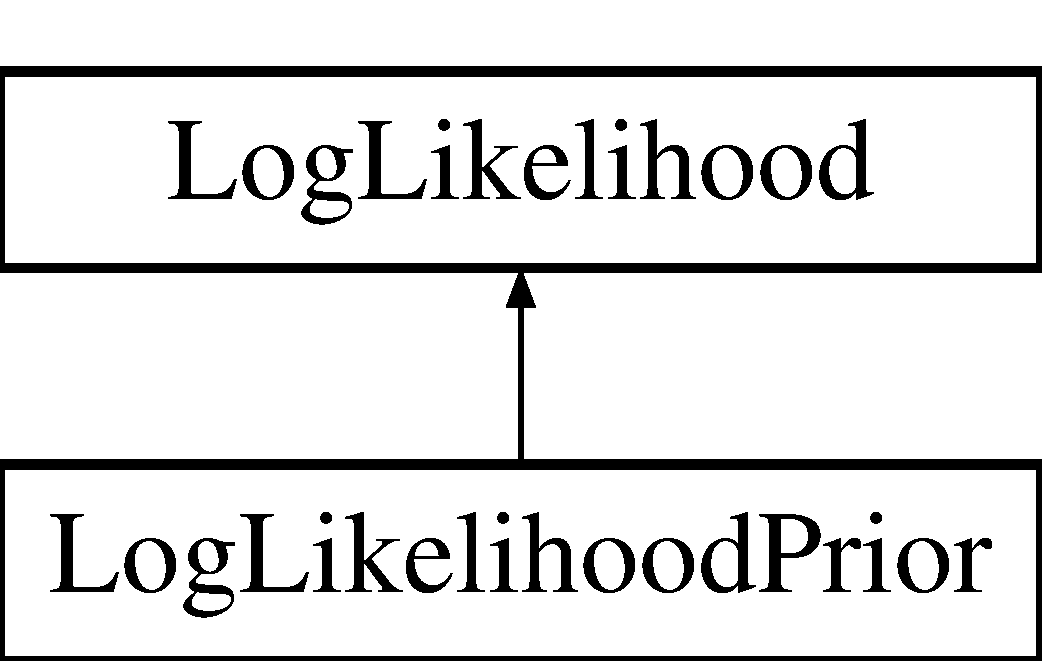
\includegraphics[height=2.000000cm]{classLogLikelihood}
\end{center}
\end{figure}
\subsection*{Public Member Functions}
\begin{DoxyCompactItemize}
\item 
\hyperlink{classLogLikelihood_a677cb07d3097385392fe49944e522858}{Log\+Likelihood} (const std\+::vector$<$ std\+::vector$<$ \hyperlink{classStar}{Star} $>$$>$ \&data, int id)
\begin{DoxyCompactList}\small\item\em Constructor function. \end{DoxyCompactList}\item 
void \hyperlink{classLogLikelihood_a748d75e2eb89965246436eb6a9274004}{Calculate} (const std\+::vector$<$ double $>$ \&position, int batch\+ID, int effective\+Batches, int max\+Batches)
\end{DoxyCompactItemize}
\subsection*{Data Fields}
\begin{DoxyCompactItemize}
\item 
\mbox{\Hypertarget{classLogLikelihood_a97ff9863958ffb93e74da07721a30cc6}\label{classLogLikelihood_a97ff9863958ffb93e74da07721a30cc6}} 
double \hyperlink{classLogLikelihood_a97ff9863958ffb93e74da07721a30cc6}{Value}
\begin{DoxyCompactList}\small\item\em The last-\/calculated value of the \hyperlink{classLogLikelihood_a748d75e2eb89965246436eb6a9274004}{Calculate()} function. \end{DoxyCompactList}\item 
\mbox{\Hypertarget{classLogLikelihood_af6d93b053cfdc1966318018831a849ec}\label{classLogLikelihood_af6d93b053cfdc1966318018831a849ec}} 
std\+::vector$<$ double $>$ \hyperlink{classLogLikelihood_af6d93b053cfdc1966318018831a849ec}{Gradient}
\begin{DoxyCompactList}\small\item\em The last-\/calculated gradient of the \hyperlink{classLogLikelihood_a748d75e2eb89965246436eb6a9274004}{Calculate()} function with respect to the associated {\ttfamily position} \end{DoxyCompactList}\item 
\mbox{\Hypertarget{classLogLikelihood_a3a4e3a1d76a663bca3705b471af583cc}\label{classLogLikelihood_a3a4e3a1d76a663bca3705b471af583cc}} 
int \hyperlink{classLogLikelihood_a3a4e3a1d76a663bca3705b471af583cc}{Stars\+Used}
\begin{DoxyCompactList}\small\item\em The number of stars within the last-\/called minibatch. \end{DoxyCompactList}\end{DoxyCompactItemize}
\subsection*{Protected Member Functions}
\begin{DoxyCompactItemize}
\item 
\mbox{\Hypertarget{classLogLikelihood_a323459623fea6256267c9724ceea8ec9}\label{classLogLikelihood_a323459623fea6256267c9724ceea8ec9}} 
void {\bfseries Reset} ()
\item 
\mbox{\Hypertarget{classLogLikelihood_a85c0af6993edd46373165089a11b4fb7}\label{classLogLikelihood_a85c0af6993edd46373165089a11b4fb7}} 
void {\bfseries Per\+Star\+Contribution} (int batch\+Id, int star\+ID, const std\+::vector$<$ double $>$ \&position)
\item 
\mbox{\Hypertarget{classLogLikelihood_aec7a3964705a6a48a1d18011e330d585}\label{classLogLikelihood_aec7a3964705a6a48a1d18011e330d585}} 
void {\bfseries Generate\+Ps} (const \hyperlink{classStar}{Star} $\ast$candidate, const std\+::vector$<$ double $>$ \&position)
\item 
\mbox{\Hypertarget{classLogLikelihood_ae0db177a301dbcb1ceb13575585dc2b2}\label{classLogLikelihood_ae0db177a301dbcb1ceb13575585dc2b2}} 
void {\bfseries Generate\+Contribution} (const \hyperlink{classStar}{Star} $\ast$candidate)
\item 
\mbox{\Hypertarget{classLogLikelihood_a525d4693f7231cb70405af68d2c2c6e9}\label{classLogLikelihood_a525d4693f7231cb70405af68d2c2c6e9}} 
void {\bfseries Assign\+Gradients} (const \hyperlink{classStar}{Star} $\ast$candidate)
\item 
\mbox{\Hypertarget{classLogLikelihood_a45c146d322f6a78b760383b624df66c8}\label{classLogLikelihood_a45c146d322f6a78b760383b624df66c8}} 
void {\bfseries Normal\+Contribution} (const \hyperlink{classStar}{Star} $\ast$candidate)
\item 
\mbox{\Hypertarget{classLogLikelihood_a48e99798d1bad7dc63fdf2019acc1c7b}\label{classLogLikelihood_a48e99798d1bad7dc63fdf2019acc1c7b}} 
void {\bfseries Poisson\+Contribution} (const \hyperlink{classStar}{Star} $\ast$candidate)
\item 
\mbox{\Hypertarget{classLogLikelihood_ac848d93699c16868bf4da1884fe5c45a}\label{classLogLikelihood_ac848d93699c16868bf4da1884fe5c45a}} 
void {\bfseries Exact\+Poisson\+Contribution} (const \hyperlink{classStar}{Star} $\ast$candidate)
\end{DoxyCompactItemize}
\subsection*{Protected Attributes}
\begin{DoxyCompactItemize}
\item 
\mbox{\Hypertarget{classLogLikelihood_ae89760ae57fa9e0ce5ef01c2b35cf487}\label{classLogLikelihood_ae89760ae57fa9e0ce5ef01c2b35cf487}} 
\hyperlink{classLikelihoodData}{Likelihood\+Data} \hyperlink{classLogLikelihood_ae89760ae57fa9e0ce5ef01c2b35cf487}{Data}
\begin{DoxyCompactList}\small\item\em member data \end{DoxyCompactList}\end{DoxyCompactItemize}


\subsection{Detailed Description}
This class holds the data and functions necessary to calculate log p(data $\vert$ x), where x is the provided \hyperlink{classEfficiencyVector}{Efficiency\+Vector}. The majority of the guts + internal workings of the class are hidden away in the \hyperlink{classLikelihoodData}{Likelihood\+Data}. 

\subsection{Constructor \& Destructor Documentation}
\mbox{\Hypertarget{classLogLikelihood_a677cb07d3097385392fe49944e522858}\label{classLogLikelihood_a677cb07d3097385392fe49944e522858}} 
\index{Log\+Likelihood@{Log\+Likelihood}!Log\+Likelihood@{Log\+Likelihood}}
\index{Log\+Likelihood@{Log\+Likelihood}!Log\+Likelihood@{Log\+Likelihood}}
\subsubsection{\texorpdfstring{Log\+Likelihood()}{LogLikelihood()}}
{\footnotesize\ttfamily Log\+Likelihood\+::\+Log\+Likelihood (\begin{DoxyParamCaption}\item[{const std\+::vector$<$ std\+::vector$<$ \hyperlink{classStar}{Star} $>$$>$ \&}]{data,  }\item[{int}]{id }\end{DoxyParamCaption})}



Constructor function. 


\begin{DoxyParams}{Parameters}
{\em data} & A vector of \hyperlink{classStar}{Star} objects arranged according to the minibatching schedule. \\
\hline
{\em id} & the M\+PI ID of the running process. \\
\hline
\end{DoxyParams}


\subsection{Member Function Documentation}
\mbox{\Hypertarget{classLogLikelihood_a748d75e2eb89965246436eb6a9274004}\label{classLogLikelihood_a748d75e2eb89965246436eb6a9274004}} 
\index{Log\+Likelihood@{Log\+Likelihood}!Calculate@{Calculate}}
\index{Calculate@{Calculate}!Log\+Likelihood@{Log\+Likelihood}}
\subsubsection{\texorpdfstring{Calculate()}{Calculate()}}
{\footnotesize\ttfamily void Log\+Likelihood\+::\+Calculate (\begin{DoxyParamCaption}\item[{const std\+::vector$<$ double $>$ \&}]{position,  }\item[{int}]{batch\+ID,  }\item[{int}]{effective\+Batches,  }\item[{int}]{max\+Batches }\end{DoxyParamCaption})}

The key function\+: executes a single minibatch calculation of the loglikelihood. 
\begin{DoxyParams}{Parameters}
{\em position} & The current \hyperlink{classEfficiencyVector}{Efficiency\+Vector} \\
\hline
{\em batch\+ID} & The minibatch to be executed \\
\hline
{\em effective\+Batches} & The current number of active minibatches \\
\hline
{\em max\+Batches} & The original number of active minibatches \\
\hline
\end{DoxyParams}
\begin{DoxyReturn}{Returns}
Assigns the value of L to \hyperlink{classLogLikelihood_a97ff9863958ffb93e74da07721a30cc6}{Value}, and the associated gradient to \hyperlink{classLogLikelihood_af6d93b053cfdc1966318018831a849ec}{Gradient} 
\end{DoxyReturn}


The documentation for this class was generated from the following file\+:\begin{DoxyCompactItemize}
\item 
/home/fraserj/\+Documents/\+Work/\+Gaia\+Selection\+Function/\+Code/\+Theia/src/\+Likelihood/Log\+Likelihood.\+h\end{DoxyCompactItemize}

\hypertarget{classLogLikelihoodPrior}{}\doxysection{Log\+Likelihood\+Prior Class Reference}
\label{classLogLikelihoodPrior}\index{LogLikelihoodPrior@{LogLikelihoodPrior}}
Inheritance diagram for Log\+Likelihood\+Prior\+:\begin{figure}[H]
\begin{center}
\leavevmode
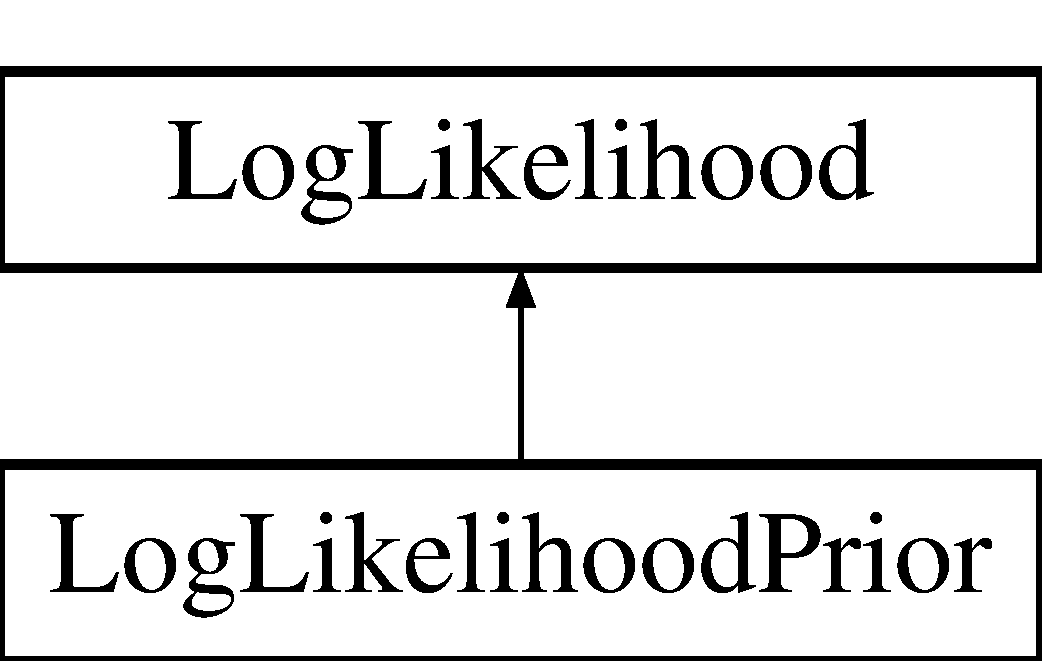
\includegraphics[height=2.000000cm]{classLogLikelihoodPrior}
\end{center}
\end{figure}
\doxysubsection*{Public Member Functions}
\begin{DoxyCompactItemize}
\item 
\mbox{\Hypertarget{classLogLikelihoodPrior_a5aa0180264b8be7d7f4bf842bf3fc763}\label{classLogLikelihoodPrior_a5aa0180264b8be7d7f4bf842bf3fc763}} 
{\bfseries Log\+Likelihood\+Prior} (const std\+::vector$<$ std\+::vector$<$ \mbox{\hyperlink{classStar}{Star}} $>$$>$ \&data, int id)
\item 
\mbox{\Hypertarget{classLogLikelihoodPrior_ac3213ddda043b381b0175ffd89445180}\label{classLogLikelihoodPrior_ac3213ddda043b381b0175ffd89445180}} 
void {\bfseries Transform\+Prior} (const std\+::vector$<$ double $>$ \&Transform\+Position, double $\ast$current\+Value, std\+::vector$<$ double $>$ \&Transform\+Gradient, int effective\+Batches, bool space, bool time, bool hyper)
\item 
\mbox{\Hypertarget{classLogLikelihoodPrior_ae3178e88d84bd9602a451d5742bc3538}\label{classLogLikelihoodPrior_ae3178e88d84bd9602a451d5742bc3538}} 
void {\bfseries Raw\+Prior} (const Eigen\+::\+Vector\+Xd \&Raw\+Params, double $\ast$current\+Value, std\+::vector$<$ double $>$ $\ast$current\+Gradient, int effective\+Batches, bool space, bool time, bool hyper)
\item 
\mbox{\Hypertarget{classLogLikelihoodPrior_a218acdef04bef419aebc1f5870469b42}\label{classLogLikelihoodPrior_a218acdef04bef419aebc1f5870469b42}} 
void {\bfseries Make\+Covariance\+Matrix} ()
\end{DoxyCompactItemize}
\doxysubsection*{Data Fields}
\begin{DoxyCompactItemize}
\item 
\mbox{\Hypertarget{classLogLikelihoodPrior_a26006b4353f2d1983cfd936f1969953c}\label{classLogLikelihoodPrior_a26006b4353f2d1983cfd936f1969953c}} 
bool {\bfseries Kg\+\_\+decomposed} = false
\item 
\mbox{\Hypertarget{classLogLikelihoodPrior_a5b64d5b52eec4a6ab6b42345c77ba7f2}\label{classLogLikelihoodPrior_a5b64d5b52eec4a6ab6b42345c77ba7f2}} 
Eigen\+::\+Matrix$<$ double, Nm, Nm $>$ {\bfseries Cholesky\+Kg}
\item 
\mbox{\Hypertarget{classLogLikelihoodPrior_ac4567245e5f7eaa048016dbb3c7ebac4}\label{classLogLikelihoodPrior_ac4567245e5f7eaa048016dbb3c7ebac4}} 
double {\bfseries cholesky\+\_\+tol} = 1e-\/4
\item 
\mbox{\Hypertarget{classLogLikelihoodPrior_acb82f3170dc5ef9992ca3c0b1d451e08}\label{classLogLikelihoodPrior_acb82f3170dc5ef9992ca3c0b1d451e08}} 
int {\bfseries choleskyN}
\item 
\mbox{\Hypertarget{classLogLikelihoodPrior_aa0413d932c2bc78bde5b6b0d69efbaa3}\label{classLogLikelihoodPrior_aa0413d932c2bc78bde5b6b0d69efbaa3}} 
std\+::vector$<$ int $>$ {\bfseries cholesky\+\_\+u}
\item 
\mbox{\Hypertarget{classLogLikelihoodPrior_a9ee359462c406bcd3e0a851eec71ba07}\label{classLogLikelihoodPrior_a9ee359462c406bcd3e0a851eec71ba07}} 
std\+::vector$<$ int $>$ {\bfseries cholesky\+\_\+v}
\item 
\mbox{\Hypertarget{classLogLikelihoodPrior_a4af02e24015068335bd22d870b0cfb32}\label{classLogLikelihoodPrior_a4af02e24015068335bd22d870b0cfb32}} 
std\+::vector$<$ double $>$ {\bfseries cholesky\+\_\+w}
\end{DoxyCompactItemize}
\doxysubsection*{Additional Inherited Members}


The documentation for this class was generated from the following file\+:\begin{DoxyCompactItemize}
\item 
/home/jack/\+Documents/\+Work/\+Gaia\+Completeness/\+Code/\+Theia/src/\+Likelihood/Log\+Likelihood\+Prior.\+h\end{DoxyCompactItemize}

\hypertarget{structMemoryBuffer}{}\doxysection{Memory\+Buffer Struct Reference}
\label{structMemoryBuffer}\index{MemoryBuffer@{MemoryBuffer}}
\doxysubsection*{Data Fields}
\begin{DoxyCompactItemize}
\item 
\mbox{\Hypertarget{structMemoryBuffer_a9dd45cbef6dc3a2b739930e4dec409d3}\label{structMemoryBuffer_a9dd45cbef6dc3a2b739930e4dec409d3}} 
int {\bfseries Size}
\item 
\mbox{\Hypertarget{structMemoryBuffer_a86585015fa99011516592b628f70db83}\label{structMemoryBuffer_a86585015fa99011516592b628f70db83}} 
int {\bfseries Position}
\item 
\mbox{\Hypertarget{structMemoryBuffer_a4e662ae94caa8b785bd7275b895cc8fb}\label{structMemoryBuffer_a4e662ae94caa8b785bd7275b895cc8fb}} 
std\+::chrono\+::time\+\_\+point$<$ std\+::chrono\+::system\+\_\+clock $>$ {\bfseries Start\+Time}
\item 
\mbox{\Hypertarget{structMemoryBuffer_ad72781d6a1db3dfbf6c81596c8a07f00}\label{structMemoryBuffer_ad72781d6a1db3dfbf6c81596c8a07f00}} 
std\+::chrono\+::time\+\_\+point$<$ std\+::chrono\+::system\+\_\+clock $>$ {\bfseries Last\+Save\+Time}
\item 
\mbox{\Hypertarget{structMemoryBuffer_a3398f730a3eb1ae6c93b3e7df134522a}\label{structMemoryBuffer_a3398f730a3eb1ae6c93b3e7df134522a}} 
int {\bfseries Override\+Time}
\item 
\mbox{\Hypertarget{structMemoryBuffer_ab047fd7f062b4db7bd4cdfff7bdaf62c}\label{structMemoryBuffer_ab047fd7f062b4db7bd4cdfff7bdaf62c}} 
std\+::vector$<$ double $>$ {\bfseries Fs}
\item 
\mbox{\Hypertarget{structMemoryBuffer_a130230435c568e4d3af8fc2bd3223293}\label{structMemoryBuffer_a130230435c568e4d3af8fc2bd3223293}} 
std\+::vector$<$ double $>$ {\bfseries Gradnorms}
\item 
\mbox{\Hypertarget{structMemoryBuffer_a99afdaad76269c41ed13560ff1fdafb7}\label{structMemoryBuffer_a99afdaad76269c41ed13560ff1fdafb7}} 
std\+::vector$<$ double $>$ {\bfseries D\+Xs}
\item 
\mbox{\Hypertarget{structMemoryBuffer_a966ec2eb4f30c5b27bddccb16b6e1c1b}\label{structMemoryBuffer_a966ec2eb4f30c5b27bddccb16b6e1c1b}} 
std\+::vector$<$ double $>$ {\bfseries Times}
\item 
\mbox{\Hypertarget{structMemoryBuffer_ae3c426ed9ede4f5c56396efb4d124b9f}\label{structMemoryBuffer_ae3c426ed9ede4f5c56396efb4d124b9f}} 
std\+::vector$<$ int $>$ {\bfseries Mini\+Batches}
\item 
\mbox{\Hypertarget{structMemoryBuffer_aa86f98179ea101b944f96521e54c6efb}\label{structMemoryBuffer_aa86f98179ea101b944f96521e54c6efb}} 
std\+::vector$<$ int $>$ {\bfseries Epochs}
\item 
\mbox{\Hypertarget{structMemoryBuffer_a86fe83559e8e303db698259261fba8b8}\label{structMemoryBuffer_a86fe83559e8e303db698259261fba8b8}} 
std\+::vector$<$ int $>$ {\bfseries Batches}
\item 
\mbox{\Hypertarget{structMemoryBuffer_a88f57d627727f3ae12f2e8cdcef9f7f6}\label{structMemoryBuffer_a88f57d627727f3ae12f2e8cdcef9f7f6}} 
int {\bfseries Analysis\+Steps}
\item 
\mbox{\Hypertarget{structMemoryBuffer_a2c7b1ba7dda880394e9f7b68c5b553d6}\label{structMemoryBuffer_a2c7b1ba7dda880394e9f7b68c5b553d6}} 
int {\bfseries Analysis\+Size}
\item 
\mbox{\Hypertarget{structMemoryBuffer_aaa05a44d029283a092aefd582977d1bb}\label{structMemoryBuffer_aaa05a44d029283a092aefd582977d1bb}} 
std\+::vector$<$ double $>$ {\bfseries Analysis}
\end{DoxyCompactItemize}


The documentation for this struct was generated from the following file\+:\begin{DoxyCompactItemize}
\item 
/home/jack/\+Documents/\+Work/\+Gaia\+Completeness/\+Code/\+Theia/src/\+Optimizer/Optimizer\+Properties.\+h\end{DoxyCompactItemize}

\hypertarget{structOptimiserProperties}{}\section{Optimiser\+Properties Struct Reference}
\label{structOptimiserProperties}\index{Optimiser\+Properties@{Optimiser\+Properties}}
\subsection*{Data Fields}
\begin{DoxyCompactItemize}
\item 
\mbox{\Hypertarget{structOptimiserProperties_a95b49b57cd02916e840da511fa01e379}\label{structOptimiserProperties_a95b49b57cd02916e840da511fa01e379}} 
Optimiser\+Modes {\bfseries Mode}
\item 
\mbox{\Hypertarget{structOptimiserProperties_aacef8e01973bcece3214de56174778bb}\label{structOptimiserProperties_aacef8e01973bcece3214de56174778bb}} 
int {\bfseries Mini\+Batches}
\item 
\mbox{\Hypertarget{structOptimiserProperties_a8d1a326eff70cb4d8472b334e95d8b07}\label{structOptimiserProperties_a8d1a326eff70cb4d8472b334e95d8b07}} 
int {\bfseries Burn\+In\+Steps}
\item 
\mbox{\Hypertarget{structOptimiserProperties_a8c385e907134c4491e8335bda1a51c1e}\label{structOptimiserProperties_a8c385e907134c4491e8335bda1a51c1e}} 
double {\bfseries Step\+Size}
\item 
\mbox{\Hypertarget{structOptimiserProperties_a7aa5f01db46d5aa68660babb57eb4068}\label{structOptimiserProperties_a7aa5f01db46d5aa68660babb57eb4068}} 
double {\bfseries Minibatch\+Down\+Step}
\item 
\mbox{\Hypertarget{structOptimiserProperties_a6387c12bb01525748510c7e2dfed4339}\label{structOptimiserProperties_a6387c12bb01525748510c7e2dfed4339}} 
double {\bfseries Max\+Harness\+Factor}
\item 
\mbox{\Hypertarget{structOptimiserProperties_a04b7f1577650e7a618a6dce076071123}\label{structOptimiserProperties_a04b7f1577650e7a618a6dce076071123}} 
int {\bfseries Harness\+Release\+Steps}
\end{DoxyCompactItemize}


The documentation for this struct was generated from the following file\+:\begin{DoxyCompactItemize}
\item 
/home/fraserj/\+Documents/\+Work/\+Gaia\+Selection\+Function/\+Code/\+Theia/src/\+Optimizer/Optimizer\+Properties.\+h\end{DoxyCompactItemize}

\hypertarget{structOptimiserStatus}{}\doxysection{Optimiser\+Status Struct Reference}
\label{structOptimiserStatus}\index{OptimiserStatus@{OptimiserStatus}}
\doxysubsection*{Data Fields}
\begin{DoxyCompactItemize}
\item 
\mbox{\Hypertarget{structOptimiserStatus_a7d45c2a7646e88ac74e2f81131f82dd2}\label{structOptimiserStatus_a7d45c2a7646e88ac74e2f81131f82dd2}} 
bool {\bfseries Continues}
\item 
\mbox{\Hypertarget{structOptimiserStatus_a70321c01ac661dabf5b180031e9b8bb2}\label{structOptimiserStatus_a70321c01ac661dabf5b180031e9b8bb2}} 
bool {\bfseries Converged}
\item 
\mbox{\Hypertarget{structOptimiserStatus_a9fa1878474d02076b4ec867808abaa3e}\label{structOptimiserStatus_a9fa1878474d02076b4ec867808abaa3e}} 
bool {\bfseries Too\+Many\+Steps}
\item 
\mbox{\Hypertarget{structOptimiserStatus_a58d7f4f4f10a4b1059b8290b6486e0d5}\label{structOptimiserStatus_a58d7f4f4f10a4b1059b8290b6486e0d5}} 
bool {\bfseries Reached\+Grad\+Convergence}
\item 
\mbox{\Hypertarget{structOptimiserStatus_a854bfaef4df67e031069a00b6325ca86}\label{structOptimiserStatus_a854bfaef4df67e031069a00b6325ca86}} 
bool {\bfseries Reached\+Step\+Convergence}
\item 
\mbox{\Hypertarget{structOptimiserStatus_a2c0efe44cd78260c25e9e4551cfb9fa6}\label{structOptimiserStatus_a2c0efe44cd78260c25e9e4551cfb9fa6}} 
bool {\bfseries Reached\+Function\+Convergence}
\item 
\mbox{\Hypertarget{structOptimiserStatus_ab4b142d6d72ddfd87174278faa7901ae}\label{structOptimiserStatus_ab4b142d6d72ddfd87174278faa7901ae}} 
bool {\bfseries Carrying\+On\+Regardless}
\item 
\mbox{\Hypertarget{structOptimiserStatus_af46b372523642690c97fe310dd04efdb}\label{structOptimiserStatus_af46b372523642690c97fe310dd04efdb}} 
bool {\bfseries External\+Down\+Step}
\item 
\mbox{\Hypertarget{structOptimiserStatus_a29dda78a363c436d68fbd5eb342cd862}\label{structOptimiserStatus_a29dda78a363c436d68fbd5eb342cd862}} 
bool {\bfseries External\+Termination}
\end{DoxyCompactItemize}


The documentation for this struct was generated from the following file\+:\begin{DoxyCompactItemize}
\item 
/home/jack/\+Documents/\+Work/\+Gaia\+Completeness/\+Code/\+Theia/src/\+Optimizer/Optimizer\+Properties.\+h\end{DoxyCompactItemize}

\hypertarget{classOptimizer}{}\doxysection{Optimizer$<$ T $>$ Class Template Reference}
\label{classOptimizer}\index{Optimizer$<$ T $>$@{Optimizer$<$ T $>$}}
\doxysubsection*{Public Member Functions}
\begin{DoxyCompactItemize}
\item 
\mbox{\Hypertarget{classOptimizer_ac0e9c13ba2d8779c27dcf1dee8ab0306}\label{classOptimizer_ac0e9c13ba2d8779c27dcf1dee8ab0306}} 
{\bfseries Optimizer} (T \&functor)
\item 
\mbox{\Hypertarget{classOptimizer_a1a87a01f13187f0aa30e5fbed82746d4}\label{classOptimizer_a1a87a01f13187f0aa30e5fbed82746d4}} 
void {\bfseries Minimize} (Vector\+Xd \&x)
\item 
\mbox{\Hypertarget{classOptimizer_a9bd0631315cd436b781b13a893b43570}\label{classOptimizer_a9bd0631315cd436b781b13a893b43570}} 
std\+::string {\bfseries Get\+Status} ()
\item 
\mbox{\Hypertarget{classOptimizer_a5764da74cea367e4fcfb109457775925}\label{classOptimizer_a5764da74cea367e4fcfb109457775925}} 
void {\bfseries Initialise\+Speed\+Controls} (std\+::vector$<$ int $>$ sizes, std\+::vector$<$ double $>$ speeds)
\end{DoxyCompactItemize}
\doxysubsection*{Data Fields}
\begin{DoxyCompactItemize}
\item 
\mbox{\Hypertarget{classOptimizer_abe6112b42cbdc2d21d357eca8e6cddcf}\label{classOptimizer_abe6112b42cbdc2d21d357eca8e6cddcf}} 
\mbox{\hyperlink{structOptimiserStatus}{Optimiser\+Status}} {\bfseries Status}
\item 
\mbox{\Hypertarget{classOptimizer_a21a7d8f0ee189158efb5a5c45844b671}\label{classOptimizer_a21a7d8f0ee189158efb5a5c45844b671}} 
\mbox{\hyperlink{structOptimiserProperties}{Optimiser\+Properties}} {\bfseries Properties}
\item 
\mbox{\Hypertarget{classOptimizer_af7371734bfa497aeef60185738d89a8e}\label{classOptimizer_af7371734bfa497aeef60185738d89a8e}} 
\mbox{\hyperlink{structStopConditions}{Stop\+Conditions}} {\bfseries Halt\+Conditions}
\item 
\mbox{\Hypertarget{classOptimizer_aecc0f0b358ac630cc78fc40a3d737b53}\label{classOptimizer_aecc0f0b358ac630cc78fc40a3d737b53}} 
\mbox{\hyperlink{structProgressTracker}{Progress\+Tracker}} {\bfseries Progress}
\end{DoxyCompactItemize}


The documentation for this class was generated from the following file\+:\begin{DoxyCompactItemize}
\item 
/home/jack/\+Documents/\+Work/\+Gaia\+Completeness/\+Code/\+Theia/src/\+Optimizer/Manual\+Optimizer.\+h\end{DoxyCompactItemize}

\hypertarget{structProgressTracker}{}\doxysection{Progress\+Tracker Struct Reference}
\label{structProgressTracker}\index{ProgressTracker@{ProgressTracker}}
\doxysubsection*{Data Fields}
\begin{DoxyCompactItemize}
\item 
\mbox{\Hypertarget{structProgressTracker_aa531f094e8ad975dfefc47ece359592d}\label{structProgressTracker_aa531f094e8ad975dfefc47ece359592d}} 
int {\bfseries Current\+Steps}
\item 
\mbox{\Hypertarget{structProgressTracker_a6dfeb8637c85c7310af398578d221bac}\label{structProgressTracker_a6dfeb8637c85c7310af398578d221bac}} 
double {\bfseries Moving\+Average}
\item 
\mbox{\Hypertarget{structProgressTracker_ae1c6ce39fe19ccf2d99e04d84bf8c52f}\label{structProgressTracker_ae1c6ce39fe19ccf2d99e04d84bf8c52f}} 
double {\bfseries Harness}
\item 
\mbox{\Hypertarget{structProgressTracker_a278dfc52759a8b774b7df65ddd474cbb}\label{structProgressTracker_a278dfc52759a8b774b7df65ddd474cbb}} 
std\+::vector$<$ double $>$ {\bfseries Speed\+Controller}
\item 
\mbox{\Hypertarget{structProgressTracker_a972f79a55a785d579031f956e52f92e8}\label{structProgressTracker_a972f79a55a785d579031f956e52f92e8}} 
int {\bfseries Steps\+Per\+Position\+Save}
\item 
\mbox{\Hypertarget{structProgressTracker_a42a1492c36b842d23968e36c01b58b91}\label{structProgressTracker_a42a1492c36b842d23968e36c01b58b91}} 
bool {\bfseries Unique\+Position\+Saves}
\item 
\mbox{\Hypertarget{structProgressTracker_a89936bd25d378bb4c90fa278ce7cc373}\label{structProgressTracker_a89936bd25d378bb4c90fa278ce7cc373}} 
bool {\bfseries Buffer\+File\+Opened}
\item 
\mbox{\Hypertarget{structProgressTracker_a1f87aa774affb12847fdf90e912ac147}\label{structProgressTracker_a1f87aa774affb12847fdf90e912ac147}} 
std\+::string {\bfseries Save\+Location}
\item 
\mbox{\Hypertarget{structProgressTracker_a5b3ece79bcfab593be27396d393f6370}\label{structProgressTracker_a5b3ece79bcfab593be27396d393f6370}} 
int {\bfseries Hashes}
\item 
\mbox{\Hypertarget{structProgressTracker_ad0995169886380eae9bed1c416e20fe7}\label{structProgressTracker_ad0995169886380eae9bed1c416e20fe7}} 
int {\bfseries Max\+Hashes}
\item 
\mbox{\Hypertarget{structProgressTracker_aa9e165a0b18af7d137a7b7bacf7e43bd}\label{structProgressTracker_aa9e165a0b18af7d137a7b7bacf7e43bd}} 
int {\bfseries Slowdown\+Triggers}
\item 
\mbox{\Hypertarget{structProgressTracker_aa9d40fe1375a0e92aa429b8b1bf40ee6}\label{structProgressTracker_aa9d40fe1375a0e92aa429b8b1bf40ee6}} 
int {\bfseries Time\+Since\+Single\+Batch}
\end{DoxyCompactItemize}


The documentation for this struct was generated from the following file\+:\begin{DoxyCompactItemize}
\item 
/home/jack/\+Documents/\+Work/\+Gaia\+Completeness/\+Code/\+Theia/src/\+Optimizer/Optimizer\+Properties.\+h\end{DoxyCompactItemize}

\hypertarget{classStar}{}\section{Star Class Reference}
\label{classStar}\index{Star@{Star}}
\subsection*{Public Member Functions}
\begin{DoxyCompactItemize}
\item 
\mbox{\Hypertarget{classStar_aace160d83fb4be45f11ca9db7dc7d51c}\label{classStar_aace160d83fb4be45f11ca9db7dc7d51c}} 
{\bfseries Star} (const std\+::vector$<$ std\+::string $>$ \&data, int bin, const std\+::vector$<$ int $>$ \&gap\+Begins, const std\+::vector$<$ int $>$ \&gap\+Ends, bool ignore\+Gaps)
\end{DoxyCompactItemize}
\subsection*{Data Fields}
\begin{DoxyCompactItemize}
\item 
\mbox{\Hypertarget{classStar_abbd3c299046233f3e5f2cf100981e05e}\label{classStar_abbd3c299046233f3e5f2cf100981e05e}} 
unsigned short int {\bfseries n\+Measure}
\item 
\mbox{\Hypertarget{classStar_ac00a219fe6c887b16cb72e263c676ea9}\label{classStar_ac00a219fe6c887b16cb72e263c676ea9}} 
unsigned short int {\bfseries n\+Visit}
\item 
\mbox{\Hypertarget{classStar_a5d29a213dddb43a01b5058486ce6e323}\label{classStar_a5d29a213dddb43a01b5058486ce6e323}} 
unsigned int {\bfseries g\+Bin}
\item 
\mbox{\Hypertarget{classStar_aaf5c50e6d1c9905c76a0bc2922de97d0}\label{classStar_aaf5c50e6d1c9905c76a0bc2922de97d0}} 
std\+::vector$<$ unsigned int $>$ {\bfseries Time\+Series}
\end{DoxyCompactItemize}


The documentation for this class was generated from the following file\+:\begin{DoxyCompactItemize}
\item 
/home/fraserj/\+Documents/\+Work/\+Gaia\+Selection\+Function/\+Code/\+Theia/src/\+Data\+Handling/Star.\+h\end{DoxyCompactItemize}

\hypertarget{structStopConditions}{}\section{Stop\+Conditions Struct Reference}
\label{structStopConditions}\index{Stop\+Conditions@{Stop\+Conditions}}
\subsection*{Data Fields}
\begin{DoxyCompactItemize}
\item 
\mbox{\Hypertarget{structStopConditions_af2622385130b911bed2c486ae8c460ff}\label{structStopConditions_af2622385130b911bed2c486ae8c460ff}} 
int {\bfseries Max\+Steps}
\item 
\mbox{\Hypertarget{structStopConditions_a43d87fc57a46592e5ebe7eb74ed0cf9f}\label{structStopConditions_a43d87fc57a46592e5ebe7eb74ed0cf9f}} 
double {\bfseries Position\+Change\+Threshold}
\item 
\mbox{\Hypertarget{structStopConditions_a8b6e6f9c935df6006ded3a0879dd33de}\label{structStopConditions_a8b6e6f9c935df6006ded3a0879dd33de}} 
double {\bfseries Gradient\+Threshold}
\item 
\mbox{\Hypertarget{structStopConditions_adc5c6c3a77f1d2162419ba06dbfa6b03}\label{structStopConditions_adc5c6c3a77f1d2162419ba06dbfa6b03}} 
double {\bfseries Function\+Change\+Threshold}
\item 
\mbox{\Hypertarget{structStopConditions_af78938739bfb3fc5971b9cbb4e61331d}\label{structStopConditions_af78938739bfb3fc5971b9cbb4e61331d}} 
int {\bfseries Single\+Batch\+Step\+Threshold}
\item 
\mbox{\Hypertarget{structStopConditions_a4b1bfd27c0581edec18fe55ae1cdced3}\label{structStopConditions_a4b1bfd27c0581edec18fe55ae1cdced3}} 
bool {\bfseries Use\+External\+Instructions}
\item 
\mbox{\Hypertarget{structStopConditions_ac32b60d59dd9c352b5dccc54d817eb6a}\label{structStopConditions_ac32b60d59dd9c352b5dccc54d817eb6a}} 
std\+::string {\bfseries Down\+Step\+File}
\item 
\mbox{\Hypertarget{structStopConditions_ae590bf77b1deeee760750df2a11fa6d8}\label{structStopConditions_ae590bf77b1deeee760750df2a11fa6d8}} 
std\+::string {\bfseries Termination\+File}
\end{DoxyCompactItemize}


The documentation for this struct was generated from the following file\+:\begin{DoxyCompactItemize}
\item 
/home/fraserj/\+Documents/\+Work/\+Gaia\+Selection\+Function/\+Code/\+Theia/src/\+Optimizer/Optimizer\+Properties.\+h\end{DoxyCompactItemize}

\hypertarget{structVariancePopulation}{}\section{Variance\+Population Struct Reference}
\label{structVariancePopulation}\index{Variance\+Population@{Variance\+Population}}
\subsection*{Public Member Functions}
\begin{DoxyCompactItemize}
\item 
\mbox{\Hypertarget{structVariancePopulation_a0a0e089d1cc596857052c0043547adb1}\label{structVariancePopulation_a0a0e089d1cc596857052c0043547adb1}} 
{\bfseries Variance\+Population} (double fraction, std\+::vector$<$ double $>$ contributions)
\item 
\mbox{\Hypertarget{structVariancePopulation_a7328d57433a870f569cf6e2bcb12e2f3}\label{structVariancePopulation_a7328d57433a870f569cf6e2bcb12e2f3}} 
double {\bfseries Variance} (double scaling)
\item 
\mbox{\Hypertarget{structVariancePopulation_a5a54f3140bc15898d3bf57340e19b90f}\label{structVariancePopulation_a5a54f3140bc15898d3bf57340e19b90f}} 
double {\bfseries d\+VariancedN} (double scaling)
\item 
\mbox{\Hypertarget{structVariancePopulation_ad2a89f4584be76a4822005764f2f6e6c}\label{structVariancePopulation_ad2a89f4584be76a4822005764f2f6e6c}} 
double {\bfseries d\+Varianced\+Alpha} (int term, double scaling)
\item 
\mbox{\Hypertarget{structVariancePopulation_ac601ad05d66b5691ed0a4b117b60c8d7}\label{structVariancePopulation_ac601ad05d66b5691ed0a4b117b60c8d7}} 
void {\bfseries Print} (double scale)
\end{DoxyCompactItemize}
\subsection*{Public Attributes}
\begin{DoxyCompactItemize}
\item 
\mbox{\Hypertarget{structVariancePopulation_aaaa1da9b4ed3f0d460a49cd0078330eb}\label{structVariancePopulation_aaaa1da9b4ed3f0d460a49cd0078330eb}} 
double {\bfseries Fraction}
\item 
\mbox{\Hypertarget{structVariancePopulation_af81f6fdf859a22cc06de6f5bfb0ed0d0}\label{structVariancePopulation_af81f6fdf859a22cc06de6f5bfb0ed0d0}} 
std\+::vector$<$ double $>$ {\bfseries Power\+Contributions}
\end{DoxyCompactItemize}


The documentation for this struct was generated from the following file\+:\begin{DoxyCompactItemize}
\item 
/home/fraserj/\+Documents/\+Work/\+Gaia\+Selection\+Function/\+Code/\+Theia/src/\+Likelihood/Data\+Storage.\+h\end{DoxyCompactItemize}

%--- End generated contents ---

% Index
\backmatter
\newpage
\phantomsection
\clearemptydoublepage
\addcontentsline{toc}{chapter}{Index}
\printindex

\end{document}
